% -*- latex -*-
%%%%%%%%%%%%%%%%%%%%%%%%%%%%%%%%%%%%%%%%%%%%%%%%%%%%%%%%%%%%%%%%
%%%%%%%%%%%%%%%%%%%%%%%%%%%%%%%%%%%%%%%%%%%%%%%%%%%%%%%%%%%%%%%%
%%%%
%%%% This text file is part of the lecture slides for
%%%% `Parallel Computing'
%%%% by Victor Eijkhout, copyright 2012-9
%%%%
%%%% Performance-slides.tex: MPI Performance issues
%%%%
%%%%%%%%%%%%%%%%%%%%%%%%%%%%%%%%%%%%%%%%%%%%%%%%%%%%%%%%%%%%%%%%
%%%%%%%%%%%%%%%%%%%%%%%%%%%%%%%%%%%%%%%%%%%%%%%%%%%%%%%%%%%%%%%%

\begin{frame}[containsverbatim]{Overview}
  We briefly touch on issues that influence MPI performance.
\end{frame}

\sectionframe{Performance measurement}

\begin{frame}[containsverbatim]{Timers}
  MPI has a \indexterm{wall clock} timer: \indexmpishow{MPI_Wtime}
  which gives the number of seconds from a certain point in the past.

  The timer has a resolution of \indexmpishow{MPI_Wtick}

  Timers can be global
\begin{lstlisting}
int *v,flag;
MPI_Attr_get( comm, MPI_WTIME_IS_GLOBAL, &v, &flag );
if (mytid==0) printf(``Time synchronized? %d->%d\n'',flag,*v);
\end{lstlisting}
  but probably aren't.
\end{frame}

\begin{frame}[containsverbatim]{Example}
    \cverbatimsnippet{pingpong}
\end{frame}

\begin{frame}[containsverbatim]{Global timing}
  Processes don't start/end simultaneously. What does a timing result
  mean overall? Take average or maximum?

  Alternative:
  \begin{lstlisting}
    MPI_Barrier(comm)
    t = MPI_Wtime();
    // something happens here
    MPI_Barrier(comm)
    t = MPI_Wtime()-t;
  \end{lstlisting}
\end{frame}

\begin{frame}[containsverbatim]{Profiling}
  See other lecture: 
  MPIP, TAU, et cetera.
\end{frame}

\begin{frame}[containsverbatim]{Your own profiling interface}
  Every routine \n{MPI_Something} calls a routine \n{PMPI_Something} that 
  does the actual work. You can now write your \n{MPI_...} routine
  which calls \indexmpishow{PMPI_...}, and inserting your own profiling calls.

  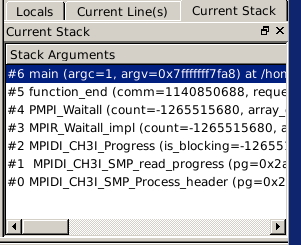
\includegraphics[scale=.7]{graphics/pmpi}
\end{frame}

\sectionframe{Programming for performance}

\begin{frame}[containsverbatim]{Eager limit}
  \begin{itemize}
  \item Optimization for small messages: bypass rendez-vous protocol
    (slide~\ref{sl:rendezvous})
  \item Cross-over point: `Eager limit'.
  \item Force efficient messages by increasing the eager limit.
  \item Beware: decreasing payoff for large messages, and
  \item Beware: buffers for eager send eat into your available memory.
  \end{itemize}
\end{frame}

\begin{frame}[containsverbatim]{Eager limit setting}
    \begin{itemize}
    \item For Intel MPI: \n{I_MPI_EAGER_THRESHOLD}
    \item mvapich2: \n{MV2_IBA_EAGER_THRESHOLD}
    \item OpenMPI: \n{OpenMPI} the
      \texttt{--mca} options \indextermtt{btl_openib_eager_limit} and
      \indextermtt{btl_openib_rndv_eager_limit}.
    \end{itemize}
\end{frame}

\begin{frame}[containsverbatim]{Blocking versus non-blocking}
  \begin{itemize}
  \item Non-blocking sends \n{MPI_Isend}/\n{Irecv} can be more
    efficient than blocking
  \item Also: allow overlap computation/communication (latency hiding)
  \item However: can usually not be considered a replacement.
  \end{itemize}
\end{frame}

\begin{frame}[containsverbatim]{Progress}
  MPI is not magically active in the background, so latency hiding is
  not automatic. Same for passive target synchronization and
  non-blocking barrier completion.
  \begin{itemize}
  \item Dedicated communications processor or thread.\\
    This is implementation dependent; for instance,
    Intel MPI: \n{I_MPI_ASYNC_PROGRESS_...} variables.
  \item Force progress by occasional calls to a polling
    routine such as \indexmpishow{MPI_Iprobe}.
  \end{itemize}
\end{frame}

\begin{frame}[containsverbatim]{Persistent sends}
  If a communication between the same pair of processes, involving the
  same buffer, happens regularly, it is possible to set up a
  \indextermsub{persistent}{communication}.

  \n{MPI_Send_init}, \n{MPI_Recv_init}, \n{MPI_Start}
\end{frame}

\begin{frame}[containsverbatim]{Buffering}

  \begin{itemize}
  \item MPI has internal buffers: copying costs performance
  \item Use your own buffer: \n{MPI_Buffer_attach}, \n{MPI_Bsend}
  \item Copying is also a problem for derived datatypes.
  \end{itemize}
\end{frame}

\begin{frame}[containsverbatim]{Graph topology and neighborhood collectives}
  \begin{itemize}
  \item Mapping problem to architecture sometimes not trivial
  \item Load balancers: \indexterm{ParMetis}, \indexterm{Zoltan}
  \item Graph topologies: \n{MPI_Dist_graph_adjacent}:\\
    allowed to reorder ranks for proximity
  \item Neighborhood collectives: \n{MPI_Neighbor_allgather_v}\\
    allow MPI to schedule optimally.
  \end{itemize}
\end{frame}

\begin{frame}[containsverbatim]{Network issues}
  Network contention means that
  \begin{itemize}
  \item Your messages can collide with other jobs
  \item messages within your job can collide
  \end{itemize}
\end{frame}

\begin{frame}{Output routing}
  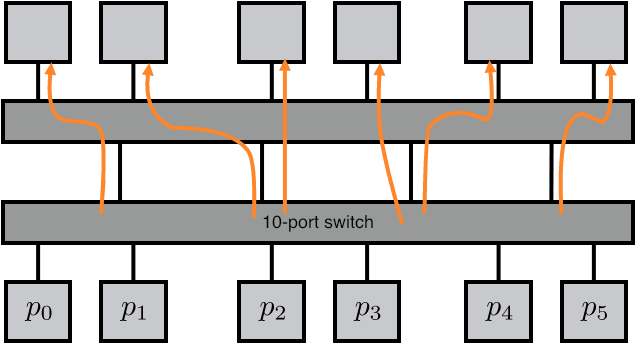
\includegraphics[scale=.4]{oversubscription}
\end{frame}

\begin{frame}{Contention}
  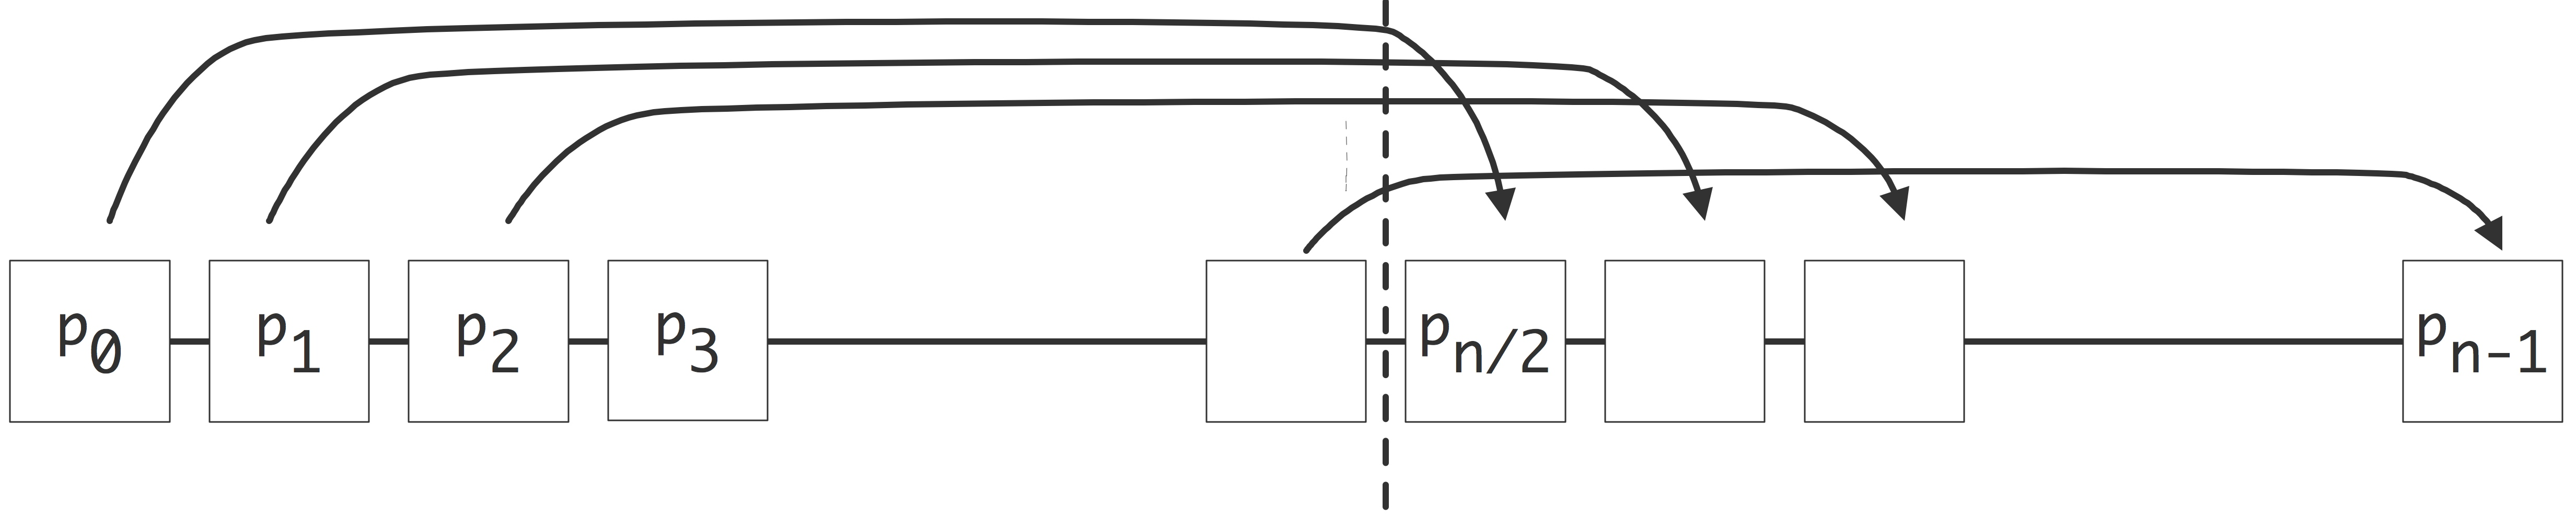
\includegraphics[scale=.4]{contention}
\end{frame}

\begin{frame}[containsverbatim]{Offloading and onloading}

  \begin{itemize}
  \item Network cards can offer assistance
  \item Mellanox: off-loading\\
    limited repertoire of scenarios where it helps
  \item Intel disagrees: on-loading
  \item Either way, investigate the capabilities of your network.
  \end{itemize}
\end{frame}

